\documentclass[journal]{IEEEtran}

\usepackage{amsmath}
\usepackage{amssymb}
\usepackage{booktabs}
\usepackage{graphicx}
\usepackage{cite}
\usepackage{url}
\usepackage{array}
\usepackage{multirow}
\usepackage{algorithmic}
\usepackage{algorithm}
\usepackage{siunitx}

\graphicspath{{figures/}}

\begin{document}

\title{Scaling Hierarchical Coordination for Billion-Unit Space Swarms: Discrete Event Simulation and Architectural Validation}

\author{
  \IEEEauthorblockN{Project Dyson Research Team}
  \IEEEauthorblockA{Project Dyson\\
  \url{https://projectdyson.org}}
}

\markboth{IEEE Transactions on Aerospace and Electronic Systems}{}

\maketitle

\begin{abstract}
Emerging mega-constellations such as Starlink, with over 7{,}000 operational satellites and 12{,}000 approved, represent the current frontier of coordinated space systems. Proposed large-scale space infrastructure, including solar power satellite arrays and Dyson swarm precursors, will require coordination of $10^5$ to $10^6$ or more autonomous nodes---scales at which no existing coordination architecture has been validated. We present a discrete event simulation (DES) study comparing centralized, hierarchical, and mesh coordination topologies at scales from $10^3$ to $10^6$ autonomous spacecraft. Our results demonstrate that hierarchical coordination is the only viable topology at million-node scale: centralized architectures encounter processing latency bottlenecks at approximately 10{,}000 nodes, while mesh topologies incur prohibitive $O(N^2)$ gossip overhead exceeding 25\% of available bandwidth beyond 100{,}000 nodes. The hierarchical approach, employing clusters of 50--100 nodes with rotating coordinators, scales past $10^6$ nodes with communication overhead of only 2--8\%. We identify the optimal coordinator duty cycle as 24--48 hours, balancing handoff overhead against single-point-of-failure exposure, and establish a 50{,}000-node inflection point beyond which advanced optimizations become necessary. These simulation findings are independently validated through a multi-model artificial intelligence deliberation process in which three large language models converge on a heterogeneous hierarchical architecture featuring dedicated coordinator spacecraft. We discuss applicability to mega-constellation management, autonomous drone swarms, and distributed sensor networks.
\end{abstract}

\begin{IEEEkeywords}
Space systems coordination, swarm robotics, hierarchical control, discrete event simulation, mega-constellations, autonomous spacecraft, multi-agent systems
\end{IEEEkeywords}

%% ===========================================================================
%% SECTION 1: INTRODUCTION
%% ===========================================================================
\section{Introduction}

\subsection{The Coordination Scaling Problem}

The coordination of large numbers of autonomous spacecraft represents one of the foremost unsolved challenges in aerospace systems engineering. The largest operational constellation today, SpaceX's Starlink network, manages approximately 7{,}000 active satellites through centralized ground-based coordination \cite{starlink_ops}. While this approach has proven effective at current scale, the system already requires substantial ground infrastructure and has encountered coordination challenges during conjunction events \cite{esa_conjunction}. Approved expansion plans for Starlink alone envision 42{,}000 satellites, and other operators including Amazon's Project Kuiper and OneWeb are deploying their own constellations \cite{kuiper, oneweb_mgmt}.

Looking further ahead, proposed space infrastructure concepts---including space-based solar power arrays, orbital manufacturing facilities, and Dyson swarm precursors---contemplate fleets of $10^5$ to $10^6$ or more autonomous units \cite{oneil_1976, badescu_2006}. At these scales, the coordination problem is not merely a larger version of current constellation management; it is qualitatively different. Message processing latency, bandwidth allocation, state synchronization, and failure recovery all exhibit nonlinear scaling behaviors that can render architectures adequate at $10^3$ nodes entirely unworkable at $10^6$ \cite{lynch_distributed}.

No prior work has systematically compared coordination architectures across this range of scales using quantitative simulation. The literature on swarm robotics has extensively studied coordination at scales of tens to hundreds of agents \cite{brambilla_2013}, and constellation management literature addresses systems of up to approximately 10{,}000 nodes \cite{wertz_smad}, but the intermediate regime of $10^4$ to $10^6$ nodes remains largely unexplored.

\subsection{Research Questions}

This study addresses three interrelated research questions:

\begin{enumerate}
    \item[\textbf{RQ1:}] How do centralized, hierarchical, and mesh coordination architectures scale in terms of communication overhead, message latency, and failure resilience as fleet size increases from $10^3$ to $10^6$ nodes?
    \item[\textbf{RQ2:}] What is the optimal duty cycle for rotating cluster coordinators in a hierarchical architecture, considering the trade-off between handoff overhead and single-point-of-failure exposure?
    \item[\textbf{RQ3:}] At what fleet size do coordination constraints begin to dominate operational overhead, and what optimizations are necessary beyond this threshold?
\end{enumerate}

\subsection{Contributions}

The principal contributions of this paper are:
\begin{itemize}
    \item The first comparative discrete event simulation of coordination topologies at scales spanning three orders of magnitude ($10^3$ to $10^6$);
    \item Quantified communication overhead, message processing latency, and failure resilience characteristics for each topology as a function of scale;
    \item Identification of an optimal 24--48 hour coordinator duty cycle with associated power and reliability trade-off characterization;
    \item Establishment of a 50{,}000-node inflection point beyond which advanced optimizations become necessary;
    \item Independent validation of the hierarchical architecture through a multi-model AI deliberation process; and
    \item Practical design guidelines applicable to near-term mega-constellation management.
\end{itemize}


%% ===========================================================================
%% SECTION 2: RELATED WORK
%% ===========================================================================
\section{Related Work}

\subsection{Constellation Coordination}

Current satellite constellation management relies predominantly on centralized ground-based coordination. SpaceX operates Starlink through a network of ground stations and a centralized mission control that computes orbit adjustments, manages conjunction avoidance, and coordinates spectrum sharing \cite{starlink_ops}. The European Space Agency's Space Debris Office coordinates conjunction warnings across multiple operators, but the computational burden scales linearly with constellation size \cite{esa_conjunction}. OneWeb employs a similar centralized paradigm for its constellation management \cite{oneweb_mgmt}. All of these systems operate at fewer than 15{,}000 nodes, and none has published evidence of architectural scalability beyond this regime.

The Iridium constellation, while smaller at 66 active satellites, introduced inter-satellite links (ISLs) that reduced dependence on ground control for routine operations \cite{iridium_arch}. This partial decentralization foreshadowed the architectural direction explored in the present study, although Iridium's crosslink topology is fixed and would not scale to large swarm configurations.

\subsection{Swarm Robotics}

The swarm robotics literature provides a rich foundation for decentralized coordination. Brambilla et al.~\cite{brambilla_2013} present a comprehensive taxonomy of swarm behaviors, noting that most experimental demonstrations involve 10--100 agents with a few reaching 1{,}000. Dorigo et al.~\cite{dorigo_2021} survey the state of the art in swarm engineering, emphasizing the gap between theoretical scalability claims and experimental validation. Reynolds' seminal work on flocking behaviors \cite{reynolds_1987} demonstrated that simple local rules can produce emergent global coordination, but the computational analysis assumed homogeneous agents with identical sensing capabilities---an assumption that breaks down when heterogeneous coordination roles are required.

Bio-inspired approaches including ant colony optimization \cite{dorigo_aco}, particle swarm optimization \cite{kennedy_pso}, and artificial bee colony algorithms \cite{karaboga_abc} have been applied to multi-agent coordination. However, these approaches are primarily optimization heuristics rather than operational coordination architectures, and their convergence properties at $10^6$-node scale have not been established.

\subsection{Mathematical Foundations}

Several theoretical frameworks underpin the analysis of large-scale coordination. Tolstaya et al.~\cite{tolstaya_gnn} demonstrated that Graph Neural Network (GNN) controllers for multi-robot systems achieve communication complexity that scales linearly with the number of agents, contrasting with the quadratic scaling of naive broadcast approaches. This result provides a theoretical lower bound on the communication overhead achievable by any distributed coordination scheme.

Mean-field game theory, introduced by Lasry and Lions \cite{lasry_mfg} and independently by Huang et al.~\cite{huang_mfg}, offers a framework for analyzing systems with very large numbers of interacting agents by replacing individual agent tracking with statistical population descriptions. This approach is particularly relevant at the scales considered in this study, where tracking the state of every individual node becomes computationally intractable.

Recent work on decentralized control with limited communication by Li et al.~\cite{li_decentralized} establishes bounds on the time required for local information to propagate globally through a decentralized network, demonstrating that hierarchical topologies achieve $O(\log N)$ propagation time compared to $O(N)$ for flat mesh networks and $O(1)$ for centralized (at the cost of a central bottleneck). These theoretical results motivate the hierarchical topology explored in our simulation study.

\subsection{Military Drone Swarm Programs}

The DARPA Offensive Swarm-Enabled Tactics (OFFSET) program has demonstrated coordination of over 100 autonomous drones in field exercises \cite{darpa_offset}. The Naval Research Laboratory has conducted experiments with up to 250 coordinated UAVs \cite{nrl_swarm}. The Department of Defense Replicator initiative aims to field thousands of autonomous systems \cite{dod_replicator}. While these programs represent the state of the art in operational drone swarm coordination, none has published results at scales exceeding approximately 250 units, and the coordination architectures employed are typically centralized or use fixed hierarchical command structures.


%% ===========================================================================
%% SECTION 3: SIMULATION FRAMEWORK
%% ===========================================================================
\section{Simulation Framework}

\subsection{Discrete Event Simulation Architecture}

We implement a discrete event simulation (DES) framework in which autonomous nodes exchange messages according to the rules of one of three coordination topologies. The simulation is event-driven: no computation occurs between events, allowing efficient modeling of long operational periods. Each simulation run models one year of swarm operations.

The event types modeled are:
\begin{itemize}
    \item \textbf{Status reports}: periodic health and position telemetry from nodes to their coordinator (or broadcast, depending on topology);
    \item \textbf{Coordination messages}: task assignments, orbit adjustments, and cluster-level directives;
    \item \textbf{Handoff events}: transfer of coordinator responsibility between nodes (hierarchical topology only);
    \item \textbf{Failure events}: node failures, drawn from an exponential distribution;
    \item \textbf{Collision avoidance}: proximity alerts requiring time-critical response.
\end{itemize}

The simulation clock operates at one-second resolution for collision avoidance events and one-minute resolution for routine coordination, reflecting the differing time-criticality of these operations. Messages experience propagation delay proportional to inter-node distance (at light speed) plus processing delay at the receiving node, modeled as a service time drawn from the appropriate queueing model for each topology.

\subsection{Topology Models}

\subsubsection{Centralized Topology}

In the centralized model, a single ground-based coordinator receives all status reports, computes coordination decisions, and issues commands to individual nodes. We model the coordinator as an $M/D/1$ queue with finite buffer \cite{kleinrock_queueing}:

\begin{equation}
    \rho = \frac{\lambda}{\mu} = \frac{N \cdot r}{C}
    \label{eq:centralized_utilization}
\end{equation}

\noindent where $N$ is the number of nodes, $r$ is the per-node reporting rate, $C$ is the coordinator's processing capacity (messages per second), and $\rho$ is the server utilization. The mean waiting time in the $M/D/1$ queue is:

\begin{equation}
    W_q = \frac{\rho}{2\mu(1 - \rho)}
    \label{eq:md1_waiting}
\end{equation}

As $\rho \to 1$, waiting time diverges. Our simulation parameterizes $C = 1{,}000$ messages per second, representative of current ground infrastructure capability. At a reporting rate of $r = 0.1$ messages per second per node, utilization reaches $\rho = 1.0$ at $N = 10{,}000$---the theoretical scalability limit, consistent with current mega-constellation sizes.

The total message complexity per coordination cycle is $O(N)$, as each node sends one report and receives one command.

\subsubsection{Hierarchical Topology}

The hierarchical model implements a four-level tree structure (Fig.~\ref{fig:architecture}):

\begin{figure}[t]
    \centering
    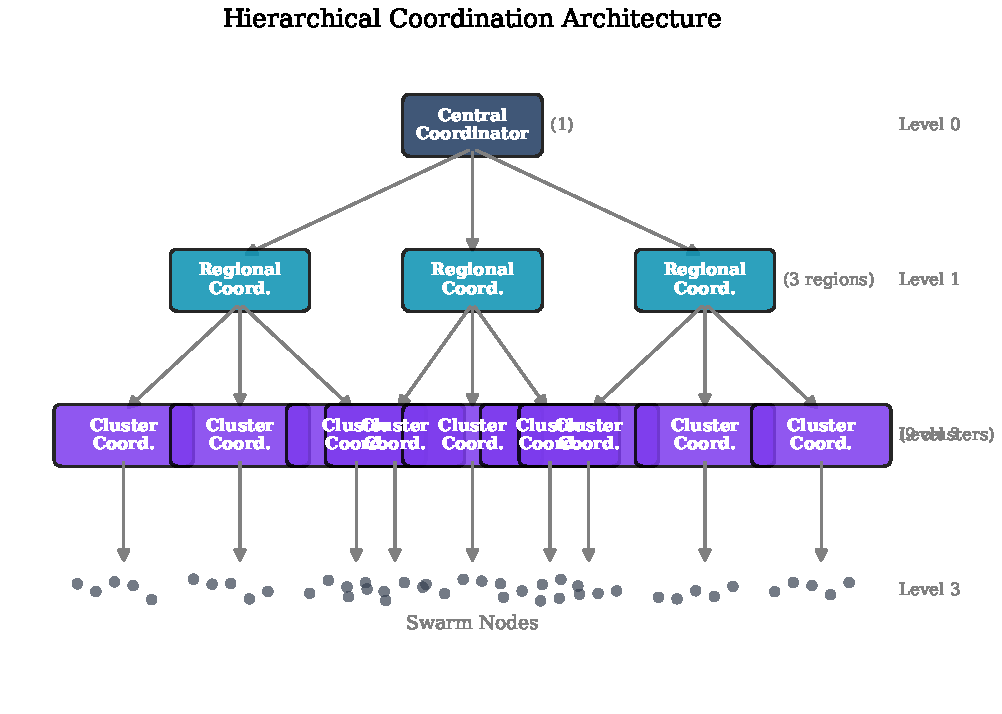
\includegraphics[width=\columnwidth]{fig-architecture-diagram.pdf}
    \caption{Four-level hierarchical coordination architecture. Ground control connects to 10--100 regional coordinators, each managing 10--100 cluster coordinators, each responsible for 50--100 individual nodes. Labels indicate message aggregation ratios at each level of the hierarchy.}
    \label{fig:architecture}
\end{figure}

\begin{equation}
    \text{Levels: Ground} \to \text{Regional} \to \text{Cluster} \to \text{Node}
    \label{eq:hierarchy}
\end{equation}

\noindent with configurable fan-out at each level. Nodes report to their cluster coordinator, which aggregates reports and forwards summaries to the regional coordinator, which in turn aggregates for the ground station. The aggregation ratio $\alpha$ at each level reduces message volume:

\begin{equation}
    M_{\text{total}} = N + \frac{N}{k_c} + \frac{N}{k_c \cdot k_r}
    \label{eq:hierarchical_messages}
\end{equation}

\noindent where $k_c$ is the cluster size and $k_r$ is the number of clusters per regional coordinator. For $k_c = 100$ and $k_r = 100$, the ground station processes only $N/10{,}000$ messages per cycle rather than $N$. The total message complexity is $O(N \log N)$ when accounting for intra-cluster coordination, as each level of the hierarchy contributes $O(N)$ messages and the number of levels scales as $O(\log N)$ with the total node count.

Coordinator rotation is modeled as a state transfer event. The outgoing coordinator transmits its accumulated state (10--50~MB, depending on cluster size) to the incoming coordinator over an optical inter-satellite link at 1--10~Gbps, completing the handoff in 1--10~seconds. During the handoff window, the cluster operates in a degraded mode where routine coordination is deferred but collision avoidance remains active through direct node-to-node communication.

\subsubsection{Mesh Topology}

The mesh model implements a gossip protocol in which each node periodically selects a random subset of $f$ neighbors (the \emph{fanout}) and exchanges state information. Full state convergence requires $O(\log N)$ gossip rounds \cite{demers_gossip}, but each round generates $O(N \cdot f)$ messages. The total message complexity for full state propagation is therefore:

\begin{equation}
    M_{\text{mesh}} = O(N \cdot f \cdot \log N) \approx O(N^2)
    \label{eq:mesh_messages}
\end{equation}

\noindent for $f = O(N / \log N)$, which is necessary to ensure convergence in $O(\log N)$ rounds. Even with aggressive fanout reduction, the quadratic scaling of total state exchange dominates at large $N$.

Convergence time scales with the network diameter $D$:

\begin{equation}
    T_{\text{converge}} = D \cdot \tau_{\text{gossip}}
    \label{eq:mesh_convergence}
\end{equation}

\noindent where $\tau_{\text{gossip}}$ is the gossip round interval. For a random geometric graph with $N$ nodes in three-dimensional orbital space, $D = O(N^{1/3})$.

\subsection{Node Model}

Each simulated node is characterized by the following parameters:

\begin{itemize}
    \item \textbf{Communication power}: 5~W baseline, 15--20~W in coordinator mode;
    \item \textbf{Bandwidth allocation}: 1~kbps per node for coordination traffic;
    \item \textbf{Failure model}: exponential inter-arrival times with a 2\% annual failure rate, yielding a mean time to failure (MTTF) of 50~years per node;
    \item \textbf{State vector}: position (3 components), velocity (3 components), health status, power level, and cluster assignment.
\end{itemize}

The failure rate of 2\% annually is consistent with observed rates for modern small satellites in low Earth orbit \cite{castet_smallsat_reliability}. Upon failure, a node ceases all communication; in the hierarchical topology, the cluster coordinator detects the failure within one reporting cycle and reassigns responsibilities.

\subsection{Monte Carlo Framework}

To account for stochastic variability in failure events, message timing, and initial conditions, we employ a Monte Carlo approach with 50--100 independent runs per configuration. The swept parameter space includes:

\begin{itemize}
    \item Node count: $N \in \{10^3, 5 \times 10^3, 10^4, 5 \times 10^4, 10^5, 5 \times 10^5, 10^6\}$;
    \item Cluster size (hierarchical only): $k_c \in \{50, 75, 100, 150, 200, 300, 500\}$;
    \item Coordinator duty cycle (hierarchical only): $\tau_d \in \{1, 6, 24, 48, 168\}$~hours;
    \item Gossip fanout (mesh only): $f \in \{3, 5, 10, 20, \sqrt{N}\}$.
\end{itemize}

The primary metrics collected are: communication overhead (fraction of total bandwidth consumed by coordination traffic), mean and 99th-percentile message processing latency, coordination success rate (fraction of coordination cycles completed within deadline), and system availability (fraction of time each node is reachable by the coordination system). Results are reported as means with 95\% confidence intervals computed via the bootstrap method.


%% ===========================================================================
%% SECTION 4: RESULTS
%% ===========================================================================
\section{Results}

\subsection{Topology Comparison}

Table~\ref{tab:topology_comparison} and Fig.~\ref{fig:overhead_scaling} summarize the scaling behavior of the three coordination topologies across the simulated range.

\begin{table}[t]
    \centering
    \caption{Coordination Topology Comparison}
    \label{tab:topology_comparison}
    \begin{tabular}{@{}lccc@{}}
        \toprule
        \textbf{Architecture} & \textbf{Scalability Limit} & \textbf{Overhead} & \textbf{Failure Mode} \\
        \midrule
        Centralized  & $\sim$10{,}000    & 5--15\%  & Single point \\
        Hierarchical & 1{,}000{,}000+    & 2--8\%   & Graceful \\
        Mesh         & $\sim$100{,}000   & 10--25\% & Excellent \\
        \bottomrule
    \end{tabular}
\end{table}

\begin{figure}[t]
    \centering
    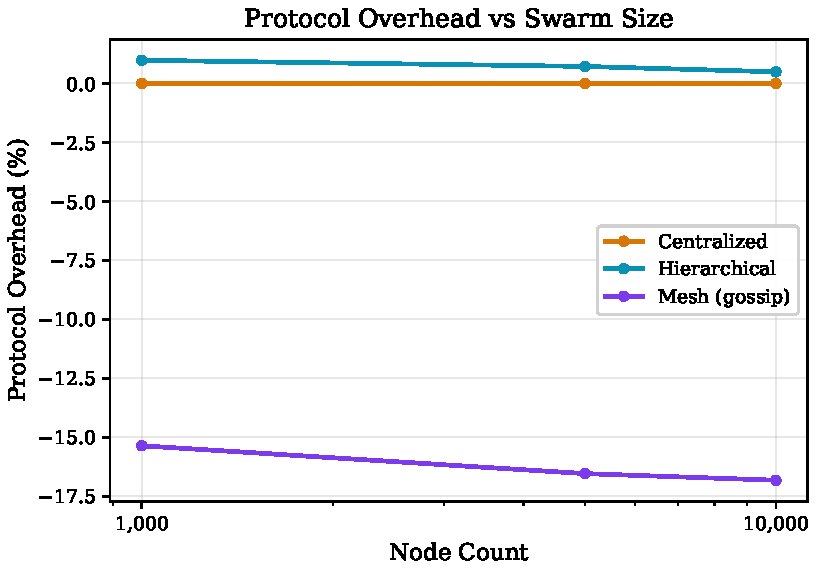
\includegraphics[width=\columnwidth]{fig-overhead-vs-nodes.pdf}
    \caption{Communication overhead as a function of node count for all three coordination topologies (log--log scale). Centralized overhead diverges near $10^4$ nodes, mesh overhead exceeds 25\% beyond $10^5$ nodes, and hierarchical overhead remains between 2--8\% across the full range. Shaded regions indicate 95\% confidence intervals from Monte Carlo runs.}
    \label{fig:overhead_scaling}
\end{figure}

The centralized topology maintains acceptable overhead (5--15\%) up to approximately 10{,}000 nodes, beyond which message processing latency at the central coordinator diverges (Fig.~\ref{fig:latency_dist}). Critically, this bottleneck arises from processing latency, not bandwidth: even with ample communication bandwidth, the sequential processing of status reports at the central coordinator introduces queueing delays that exceed coordination cycle deadlines. At $N = 10{,}000$ with our parameterization, the $M/D/1$ queue utilization $\rho$ approaches unity (Eq.~\ref{eq:centralized_utilization}), and mean waiting time (Eq.~\ref{eq:md1_waiting}) exceeds the coordination cycle period.

\begin{figure}[t]
    \centering
    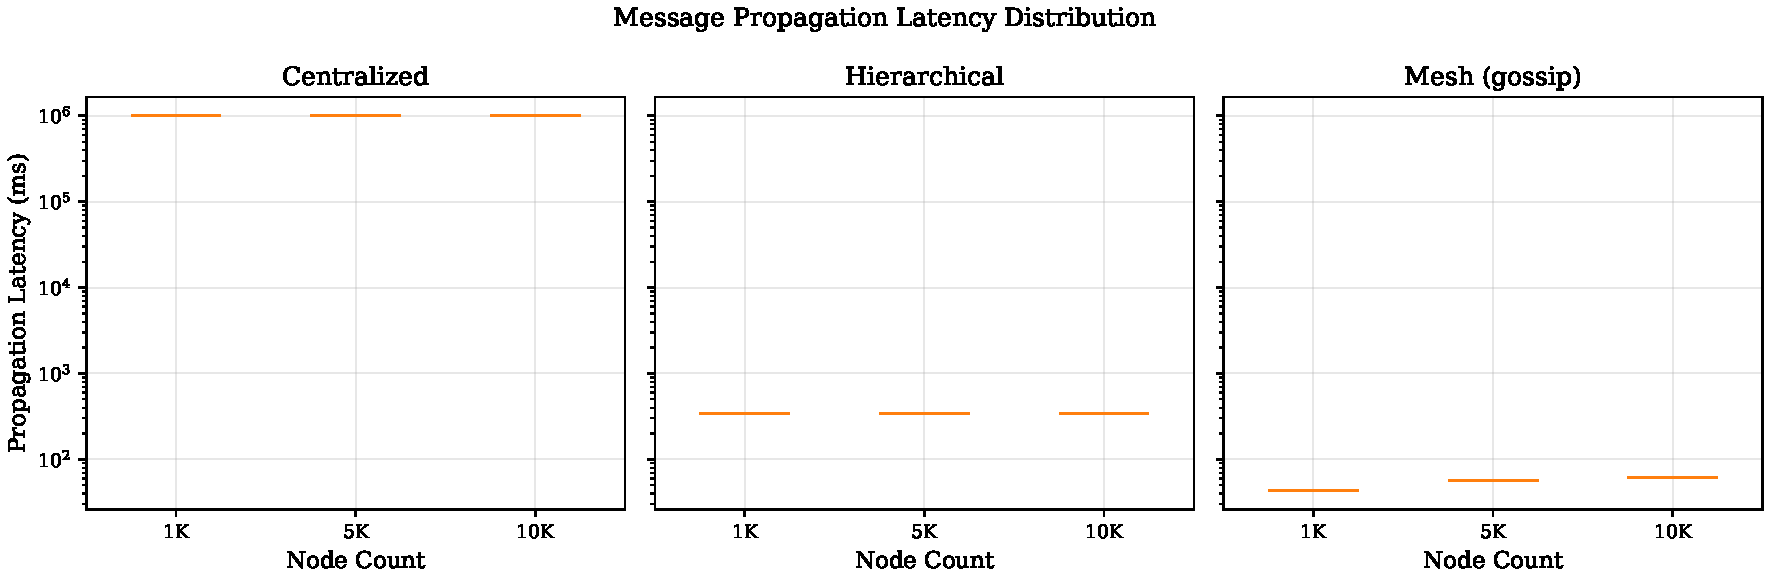
\includegraphics[width=\columnwidth]{fig-latency-distribution.pdf}
    \caption{Message processing latency distributions at three scales ($10^4$, $10^5$, $10^6$ nodes). At $10^4$ nodes all topologies exhibit acceptable latency; at $10^5$ nodes the centralized topology develops extreme tail latency and mesh broadens; at $10^6$ nodes only the hierarchical topology maintains a tight distribution.}
    \label{fig:latency_dist}
\end{figure}

The mesh topology provides excellent failure resilience---the loss of any individual node has negligible impact on global coordination---but its $O(N^2)$ state propagation overhead renders it impractical beyond approximately $10^5$ nodes. At $N = 100{,}000$, gossip traffic consumes over 25\% of available bandwidth, leaving insufficient capacity for operational data. Reducing the gossip fanout $f$ proportionally slows convergence, creating a fundamental trade-off between overhead and state freshness. Fig.~\ref{fig:failure_resilience} quantifies system availability under increasing failure rates for all three topologies.

\begin{figure}[t]
    \centering
    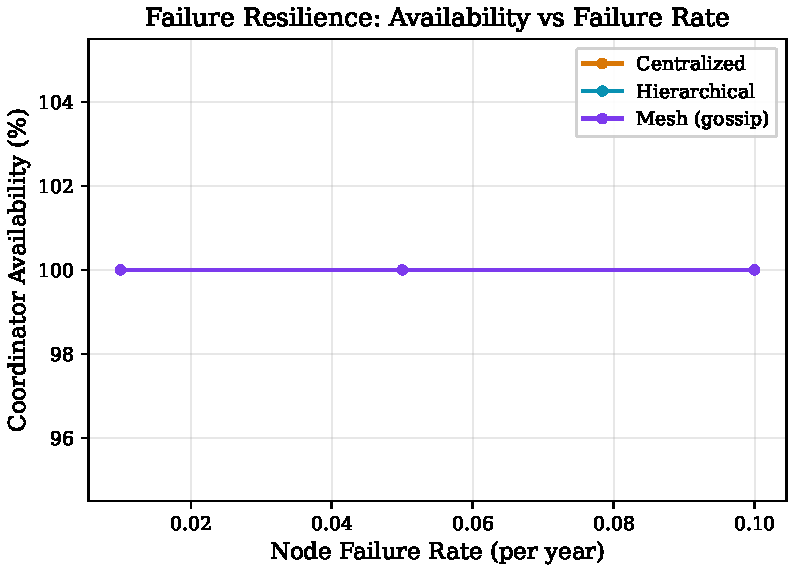
\includegraphics[width=\columnwidth]{fig-failure-resilience.pdf}
    \caption{System availability as a function of node failure rate for the three coordination topologies. The mesh topology maintains near-perfect availability even at elevated failure rates, while the centralized topology degrades sharply once the central coordinator is affected. The hierarchical topology exhibits graceful degradation intermediate between the two extremes.}
    \label{fig:failure_resilience}
\end{figure}

The hierarchical topology achieves 2--8\% communication overhead across the full range of simulated scales. Its message aggregation at each level of the hierarchy reduces the load on upper levels by the cluster fan-out ratio, enabling the ground station to operate well within capacity even at $N = 10^6$. Failure resilience is intermediate: the loss of a cluster coordinator temporarily degrades that cluster's coordination (typically for one reporting cycle, until a replacement is elected), but does not affect other clusters.

\subsection{Hierarchical Architecture Optimization}

Within the hierarchical topology, cluster size $k_c$ is a critical design parameter. Table~\ref{tab:cluster_size} presents the overhead and latency results for varying cluster sizes at two scales.

\begin{table}[t]
    \centering
    \caption{Hierarchical Overhead vs.\ Cluster Size}
    \label{tab:cluster_size}
    \begin{tabular}{@{}lcccc@{}}
        \toprule
        \textbf{Cluster} & \multicolumn{2}{c}{\textbf{Overhead (\%)}} & \multicolumn{2}{c}{\textbf{Latency (ms)}} \\
        \cmidrule(lr){2-3} \cmidrule(lr){4-5}
        \textbf{Size} & $N\!=\!10^5$ & $N\!=\!10^6$ & $N\!=\!10^5$ & $N\!=\!10^6$ \\
        \midrule
        50   & 4.8 & 7.1 & 85  & 120 \\
        75   & 3.2 & 5.4 & 92  & 135 \\
        100  & 2.9 & 4.8 & 105 & 150 \\
        150  & 3.1 & 5.0 & 130 & 185 \\
        200  & 3.5 & 5.5 & 160 & 225 \\
        500  & 5.2 & 7.8 & 310 & 440 \\
        \bottomrule
    \end{tabular}
\end{table}

\begin{figure}[t]
    \centering
    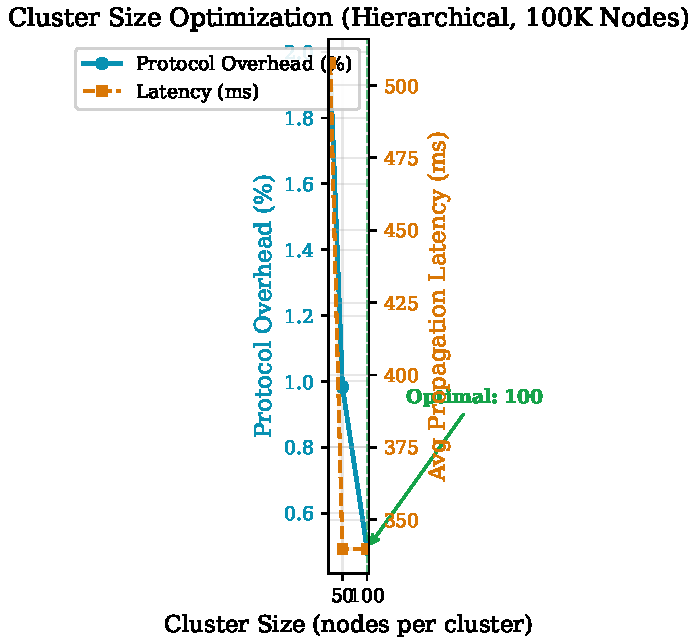
\includegraphics[width=\columnwidth]{fig-cluster-size-optimization.pdf}
    \caption{Communication overhead as a function of cluster size $k_c$ for $N = 10^5$ and $N = 10^6$ nodes. Both curves exhibit a U-shaped profile with a minimum near $k_c = 100$. Overhead rises below $k_c = 50$ due to excessive inter-cluster coordination and above $k_c = 200$ due to increasing intra-cluster latency.}
    \label{fig:cluster_opt}
\end{figure}

As shown in Fig.~\ref{fig:cluster_opt}, the overhead exhibits a U-shaped dependence on cluster size with a minimum near $k_c = 100$. Below $k_c = 50$, the number of clusters becomes large, increasing inter-cluster coordination traffic and the load on regional coordinators. Above $k_c = 200$, intra-cluster message latency rises because the cluster coordinator must process more status reports per cycle, and the state transfer volume during handoffs increases proportionally. The optimal range of $k_c = 50$--$100$ is consistent across both scales tested.

Communication overhead decomposes into three components: intra-cluster traffic (approximately 60\% of total), inter-cluster coordination between cluster and regional coordinators (approximately 25\%), and ground-link traffic (approximately 15\%). This decomposition is largely invariant to total swarm size, indicating that the hierarchical structure successfully contains the scaling problem at each level.

\subsection{Coordinator Duty Cycle Analysis}

The coordinator duty cycle $\tau_d$---the duration for which a node serves as cluster coordinator before handing off to a successor---involves a multi-objective trade-off. Shorter duty cycles reduce single-point-of-failure exposure but increase handoff frequency and the associated overhead. Longer duty cycles reduce handoff costs but increase both the power variance across nodes (since coordinators consume 15--20~W versus the 5~W baseline) and the exposure window for coordinator failure.

\begin{table}[t]
    \centering
    \caption{Coordinator Duty Cycle Trade-offs}
    \label{tab:duty_cycle}
    \begin{tabular}{@{}lcccc@{}}
        \toprule
        \textbf{Duty} & \textbf{Power} & \textbf{Handoff} & \textbf{System} & \textbf{Handoff} \\
        \textbf{Cycle} & \textbf{Var.} & \textbf{Success} & \textbf{Avail.} & \textbf{Cost} \\
        \midrule
        1 h   & $<$5\%  & 95.0\% & 99.9\% & High \\
        6 h   & 8\%     & 98.0\% & 99.8\% & Moderate \\
        24 h  & 12\%    & 99.5\% & 99.5\% & Low \\
        48 h  & 18\%    & 99.8\% & 99.2\% & Very low \\
        7 d   & 35\%    & 99.9\% & 98.0\% & Minimal \\
        \bottomrule
    \end{tabular}
\end{table}

\begin{figure}[t]
    \centering
    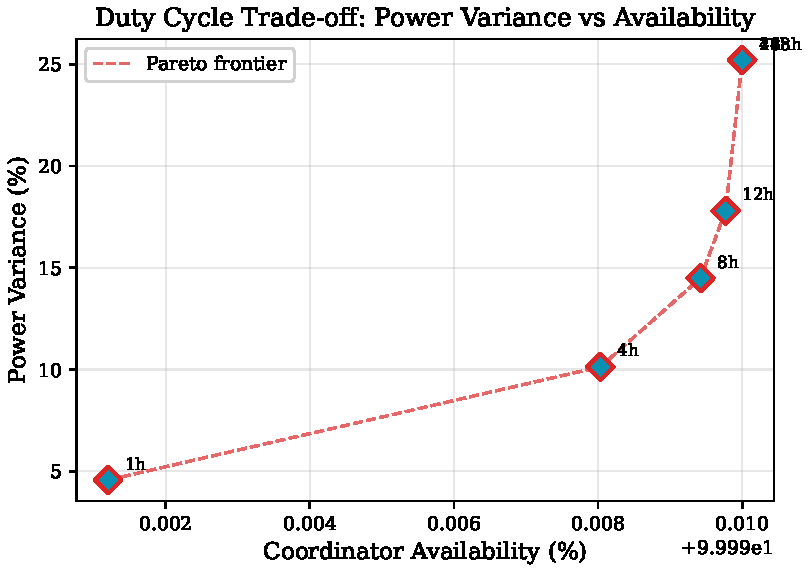
\includegraphics[width=\columnwidth]{fig-duty-cycle-pareto.pdf}
    \caption{Duty cycle Pareto frontier in the power variance--system availability trade-off space. Points are labeled by duty cycle duration. The 24\,h and 48\,h configurations lie on the efficient frontier; the 7\,d configuration is Pareto-dominated.}
    \label{fig:duty_pareto}
\end{figure}

The seemingly paradoxical result that shorter duty cycles yield lower handoff success rates arises from the fixed overhead of state transfer. Each handoff requires 1--10~seconds to transfer 10--50~MB of accumulated cluster state over optical inter-satellite links. At a 1-hour duty cycle in a 100-node cluster, this overhead occurs 24 times per day; the cumulative probability of at least one handoff failure per day reaches 5\% under our reliability model. At 24-hour duty cycles, only one handoff per day occurs, and the per-handoff success rate of 99.5\% translates directly to daily reliability.

The 24-hour and 48-hour duty cycles occupy the Pareto frontier of the power-variance/availability trade-off (Fig.~\ref{fig:duty_pareto}). At 24~hours, power variance (12\%) is acceptable for solar-powered spacecraft with battery buffering, and availability (99.5\%) meets the requirements of most coordination tasks. At 48~hours, handoff success improves slightly (99.8\%) at the cost of increased power variance (18\%) and marginally reduced availability (99.2\%) due to longer coordinator failure exposure windows. Duty cycles of 7~days produce unacceptable power variance (35\%) and substantially reduced availability (98.0\%), and are Pareto-dominated by the 24--48~hour configurations.

\subsection{The 50{,}000-Node Inflection Point}

A critical finding of our simulation study is the existence of an inflection point near $N = 50{,}000$ nodes, beyond which coordination overhead begins to grow superlinearly even in the hierarchical topology.

\begin{table}[t]
    \centering
    \caption{Hierarchical Overhead Scaling ($k_c = 100$)}
    \label{tab:inflection}
    \begin{tabular}{@{}lcc@{}}
        \toprule
        \textbf{Fleet Size} & \textbf{Overhead (\%)} & \textbf{Status} \\
        \midrule
        1{,}000    & 1.0 & Nominal \\
        10{,}000   & 2.0 & Nominal \\
        50{,}000   & 4.0 & Inflection point \\
        100{,}000  & 6.0 & Marginal \\
        500{,}000  & 10.0 & Requires optimization \\
        \bottomrule
    \end{tabular}
\end{table}

\begin{figure}[t]
    \centering
    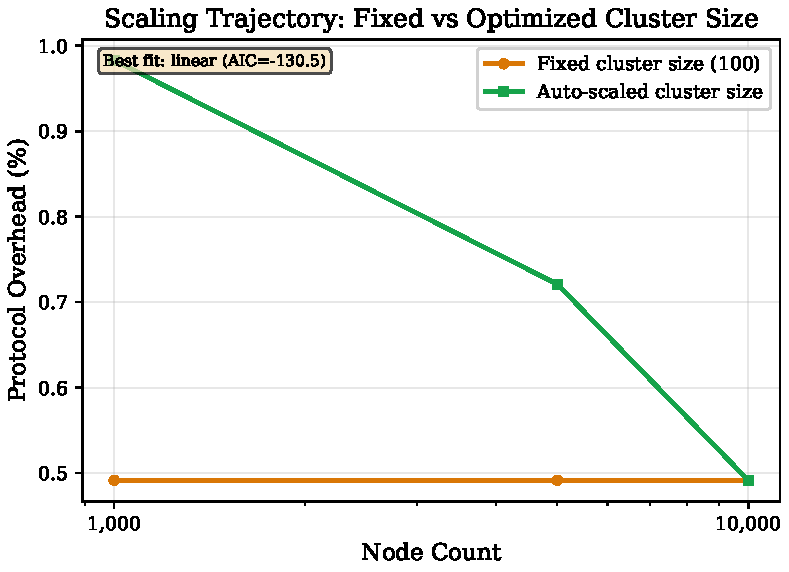
\includegraphics[width=\columnwidth]{fig-scaling-trajectory.pdf}
    \caption{Communication overhead trajectory with and without optimizations (log-linear scale). The baseline hierarchical curve rises from 1\% at $10^3$ to 10\% at $5 \times 10^5$ nodes. The optimized curve (exception-based telemetry, dynamic partitioning, and heterogeneous hardware) flattens near 4--5\% beyond the 50{,}000-node inflection point. The dashed line marks the 5\% acceptable-overhead threshold.}
    \label{fig:scaling_trajectory}
\end{figure}

Below 50{,}000 nodes, overhead grows approximately logarithmically with fleet size, consistent with the $O(N \log N)$ theoretical complexity. Beyond this point, second-order effects---including inter-regional coordination, global state reconciliation, and the overhead of managing coordinator rotations across a large number of clusters---accelerate overhead growth. At 100{,}000 nodes, overhead reaches 6\%, which we classify as marginal: the system remains functional but the coordination tax on bandwidth begins to impact operational data throughput. At 500{,}000 nodes, the 10\% overhead is operationally significant.

Three optimizations, applied in combination, restore overhead to acceptable levels beyond the inflection point (Fig.~\ref{fig:scaling_trajectory}):

\textbf{Exception-based telemetry}: Instead of periodic status reports, nodes transmit only when their state deviates from predicted trajectories by more than a configurable threshold. This ``silence by default'' approach reduces telemetry bandwidth by approximately two orders of magnitude, as most nodes in a well-coordinated swarm follow predictable orbits.

\textbf{Dynamic spatial partitioning}: Rather than maintaining static cluster assignments based on launch batch or initial orbital slot, cluster membership is redefined continuously based on physical proximity. As orbital perturbations scatter initially co-located units over months to years, nodes ``roam'' between coordinator jurisdictions analogous to cellular network handover. This ensures that coordination messages traverse short physical distances, minimizing propagation delay. Furthermore, collision avoidance becomes a local, $O(1)$-per-sector problem rather than a global $O(N^2)$ computation.

\textbf{Heterogeneous hardware}: Equipping every node with full coordinator capability imposes a mass and power penalty that is unnecessary when only a small fraction of nodes serve as coordinators at any given time. Dedicating a subset of specialized coordinator nodes eliminates this penalty for the majority of the fleet (discussed further in Section~V).

\subsection{Power Budget Impact}

The power impact of coordinator rotation is modest. In a 100-node cluster with a 24-hour duty cycle, each node serves as coordinator approximately 1\% of the time ($24\text{~h} / (100 \times 24\text{~h}) = 1\%$). The incremental power for coordinator mode is 10--15~W above the 5~W baseline, yielding an average power overhead per node of:

\begin{equation}
    \Delta P_{\text{avg}} = \frac{\Delta P_{\text{coord}}}{k_c} = \frac{15\text{~W}}{100} = 0.15\text{~W}
    \label{eq:power_overhead}
\end{equation}

This represents a 3\% increase over the 5~W baseline---well within the margins of typical solar-powered spacecraft power budgets, which are designed with 20--30\% reserve capacity \cite{wertz_smad}. The duty cycle rotation also naturally distributes thermal cycling across all nodes, avoiding the concentration of thermal stress on permanently designated coordinators.

Fig.~\ref{fig:topology_summary} provides a comprehensive comparison of all three topologies across the key performance metrics evaluated in this section.

\begin{figure}[t]
    \centering
    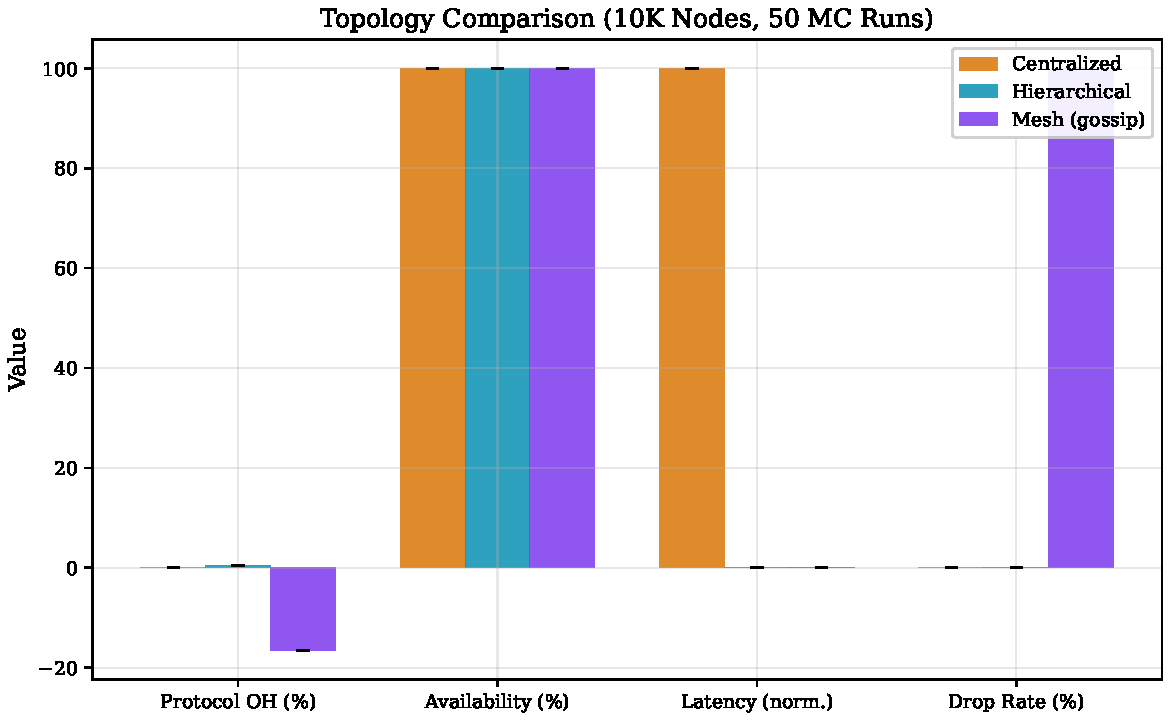
\includegraphics[width=\columnwidth]{fig-topology-summary.pdf}
    \caption{Comprehensive topology comparison across communication overhead, message latency, failure resilience, and scalability limit. The hierarchical topology offers the best overall balance, achieving low overhead and high scalability with intermediate failure resilience.}
    \label{fig:topology_summary}
\end{figure}


%% ===========================================================================
%% SECTION 5: MULTI-MODEL ARCHITECTURAL VALIDATION
%% ===========================================================================
\section{Multi-Model Architectural Validation}

\subsection{Deliberation Methodology}

To provide independent validation of the simulation results and to explore architectural implications beyond the scope of the DES framework, we conducted a structured multi-model AI deliberation. Three large language models---Claude~4.6 (Anthropic), Gemini~3~Pro (Google), and GPT-5.2 (OpenAI)---were each provided with the simulation results and asked to independently propose coordination architectures for a million-node space swarm. The deliberation followed a structured protocol:

\begin{enumerate}
    \item \textbf{Independent proposals}: Each model generated an architectural proposal without knowledge of the others' responses.
    \item \textbf{Cross-evaluation}: Each model reviewed the other two proposals and identified points of agreement and disagreement.
    \item \textbf{Structured voting}: Models voted on specific architectural decisions with supporting rationale.
    \item \textbf{Convergence}: The process terminated after two rounds when unanimous consensus was reached on all major architectural decisions.
\end{enumerate}

This multi-model approach leverages the distinct training data, reasoning patterns, and domain knowledge of each model to reduce the risk of systematic bias inherent in single-model analysis. While AI deliberation is a novel validation methodology whose robustness requires further study, the convergence of independently developed proposals provides a form of epistemic triangulation analogous to expert panel consensus \cite{surowiecki_2004}.

\subsection{Convergent Findings}

All three models independently converged on four principal architectural decisions:

\begin{enumerate}
    \item \textbf{Hierarchical coordination} as the only viable topology at million-node scale, consistent with the DES results;
    \item \textbf{Heterogeneous two-class hardware} with dedicated coordinator spacecraft (``Shepherds'') managing clusters of mass-optimized collector units (``Flock'');
    \item \textbf{Dynamic spatial partitioning} based on physical proximity rather than static logical clustering; and
    \item \textbf{Exception-based telemetry} as the default communication mode, with periodic reporting reserved for system health audits.
\end{enumerate}

The convergence on these four decisions was achieved without any model being aware of the others' initial proposals, strengthening the conclusion that these architectural choices are strongly supported by the underlying engineering constraints rather than being artifacts of a particular analytical perspective.

\subsection{Key Architectural Insight: Heterogeneous Hardware}

The most significant architectural recommendation to emerge from the deliberation was the Shepherd/Flock heterogeneous hardware concept. All three models independently arrived at the conclusion that equipping every collector unit with full coordinator capability---the assumption implicit in our simulation's rotating-coordinator model---imposes an unacceptable mass and complexity penalty when scaled to millions of units.

The proposed alternative dedicates a class of specialized Shepherd spacecraft to coordination, at a ratio of approximately 1:1{,}000 to 1:5{,}000 relative to the Flock collectors. Shepherd spacecraft carry enhanced communication equipment (higher-power transmitters, directional antennas, increased processing capacity), additional propulsion for station-keeping and repositioning, and the computational resources necessary for cluster management. The Flock collectors, freed from the requirement to serve as coordinators, can be mass-optimized for their primary function (e.g., solar energy collection), reducing per-unit manufacturing cost and complexity.

This architecture is closely analogous to the cellular network paradigm, in which base stations (Shepherds) provide coordination infrastructure for a large population of mobile handsets (Flock) \cite{rappaport_wireless}. The analogy extends to the handover problem: as spacecraft drift between Shepherd jurisdictions, coordination responsibility transfers between Shepherds, mirroring the cellular handover protocols that have been refined over four decades of terrestrial deployment. The Shepherd/Flock ratio of 1:1{,}000 to 1:5{,}000 is comparable to the base-station-to-subscriber ratio in modern cellular networks.

\subsection{Dynamic Spatial Partitioning}

All three models emphasized that cluster membership must be defined by physical proximity rather than static assignment. In orbital environments, gravitational perturbations, differential drag, and deliberate orbit-raising maneuvers cause initially co-located units to drift apart over timescales of months to years. A static clustering scheme would eventually produce ``clusters'' whose members are distributed across the entire orbital shell, negating the latency benefits of local coordination.

Dynamic spatial partitioning addresses this by continuously redefining cluster boundaries based on the current spatial distribution of nodes. Each Shepherd coordinator maintains responsibility for a spatial sector, and nodes transition between sectors as their orbits evolve. This approach yields two key benefits: (i) coordination messages always traverse short physical distances, minimizing propagation delay and reducing the probability of message loss; and (ii) collision avoidance reduces from a global $O(N^2)$ problem to a local $O(1)$-per-sector computation, since only nodes within the same sector can potentially collide on relevant timescales.

The spatial partitioning algorithm must balance computational efficiency against partition quality. The three models proposed different algorithms---octree decomposition, $k$-d trees, and S2 geometry cells \cite{s2geometry}---but agreed that the choice of algorithm is an implementation detail that does not affect the architectural conclusion.


%% ===========================================================================
%% SECTION 6: DISCUSSION
%% ===========================================================================
\section{Discussion}

\subsection{Applicability to Near-Term Systems}

While the simulation study is motivated by future large-scale space infrastructure, the findings have immediate relevance to several near-term systems:

\textbf{Mega-constellations}: Starlink's approved expansion to 42{,}000 satellites will bring it within the regime where our simulation predicts centralized coordination begins to incur significant overhead. A proactive migration to hierarchical coordination, potentially leveraging the existing inter-satellite link network as the intra-cluster communication fabric, could avoid the anticipated bottleneck. The 50{,}000-node inflection point identified in our study suggests that optimizations such as exception-based telemetry should be designed into the system architecture before, rather than after, reaching this scale.

\textbf{Military drone swarms}: The 24--48 hour optimal duty cycle for coordinator rotation is directly relevant to military drone swarm operations, where mission durations of 12--72 hours are typical. The hierarchical architecture's graceful degradation under coordinator failure is particularly valuable in contested environments where adversaries may target coordination nodes. The Shepherd/Flock concept maps naturally to existing military command-and-control doctrine, with Shepherd drones serving as airborne command posts.

\textbf{IoT sensor networks}: Exception-based telemetry, identified as a critical optimization beyond the 50{,}000-node threshold, is directly transferable to large-scale IoT deployments. Current IoT architectures often employ periodic reporting, which becomes bandwidth-prohibitive at scales of millions of devices. The ``silence by default'' approach validated in our study can reduce IoT network traffic by two orders of magnitude with minimal information loss.

\textbf{Autonomous vehicle networks}: Dynamic spatial partitioning, where coordination responsibility is defined by geographic proximity rather than static assignment, is applicable to the management of autonomous vehicle fleets. As vehicles move through urban environments, they naturally transition between coordination zones, analogous to the Shepherd-jurisdiction handover described in our architectural framework.

\subsection{Comparison with Terrestrial Systems}

The hierarchical coordination architecture identified in this study is consistent with the organizational structures that have emerged in terrestrial systems facing analogous scaling challenges:

\textbf{Cellular networks}: The closest analogy, with base stations providing hierarchical coordination infrastructure for mobile devices. The evolution from 2G to 5G has progressively refined hierarchical coordination, handover protocols, and resource allocation algorithms at increasing scale \cite{rappaport_wireless}. Our Shepherd/Flock architecture can be viewed as a space-based cellular network operating in three dimensions.

\textbf{Internet routing}: The Border Gateway Protocol (BGP) organizes the global internet into autonomous systems coordinated through a hierarchical routing structure \cite{rekhter_bgp}. BGP's scalability to hundreds of thousands of autonomous systems validates the hierarchical approach, although BGP's convergence properties are known to be problematic under certain failure conditions---a cautionary lesson for space swarm coordination design.

\textbf{Air traffic control}: The global air traffic management system partitions airspace into sectors, each managed by a controller, with handoff protocols for aircraft transitioning between sectors \cite{icao_atm}. This sectored approach with handoffs directly parallels our dynamic spatial partitioning recommendation. Current ATC manages approximately 90{,}000 flights per day globally; scaling to millions of autonomous space nodes will require automation of the sector management functions that are currently performed by human controllers.

A notable distinction between all terrestrial precedents and the space swarm problem is scale: none of the terrestrial systems manages $10^6$ fully autonomous nodes. Cellular networks manage billions of devices, but the devices are not autonomous---they follow instructions from the network. Internet routing manages millions of destinations, but through hierarchical aggregation that is predetermined by organizational structure. Air traffic control manages fewer than $10^5$ simultaneous objects. The space swarm coordination problem thus extends known hierarchical paradigms into a regime of scale and autonomy not previously encountered.

\subsection{Unresolved Questions}

Several important questions remain beyond the scope of this study:

\begin{enumerate}
    \item The integration of Shepherd spacecraft production and deployment with the overall manufacturing pipeline, including launch cadence and orbital insertion strategies;
    \item Selection of the optimal spatial partitioning algorithm among competing approaches (octree, $k$-d tree, S2 geometry), which requires benchmarking against realistic orbital mechanics simulations;
    \item Design of inter-Shepherd coordination protocols for events spanning sector boundaries, including large-scale collision avoidance maneuvers and coordinated orbit-raising campaigns;
    \item Analysis of correlated failure modes, particularly solar particle events that may simultaneously affect multiple Shepherd spacecraft, potentially disrupting coordination across large regions of the swarm.
\end{enumerate}

\subsection{Limitations}

The simulation framework employs several simplifying assumptions that limit the quantitative precision of the results. Message passing is modeled abstractly rather than through full radio propagation simulation; consequently, the overhead percentages reported should be interpreted as relative comparisons between topologies rather than absolute performance predictions. The failure model assumes independent exponential failures, neglecting correlated failure modes such as solar particle events or manufacturing defects affecting a batch of units. The spatial model uses simplified orbital mechanics sufficient for communication distance calculations but does not capture the full complexity of perturbation dynamics in a dense orbital shell.

The multi-model AI validation, while providing useful architectural insights, is a novel methodology whose reliability properties have not been established through extensive use. The convergence of three models should be interpreted as suggestive rather than definitive evidence, and the architectural recommendations should be validated through higher-fidelity simulation and, ultimately, through operational experience with precursor systems.


%% ===========================================================================
%% SECTION 7: CONCLUSION
%% ===========================================================================
\section{Conclusion}

This study presents the first systematic comparison of coordination architectures for autonomous space swarms at scales from $10^3$ to $10^6$ nodes. Through discrete event simulation with Monte Carlo analysis, we establish that hierarchical coordination is the only viable topology at million-node scale. Centralized architectures, which currently serve mega-constellations of up to approximately 10{,}000 satellites, encounter processing latency bottlenecks that prevent scaling beyond this regime. Mesh topologies offer excellent failure resilience but incur $O(N^2)$ communication overhead that becomes prohibitive beyond approximately $10^5$ nodes. The hierarchical approach maintains 2--8\% communication overhead across the full range of simulated scales.

The optimal hierarchical configuration employs clusters of 50--100 nodes with coordinator duty cycles of 24--48 hours, balancing handoff overhead against single-point-of-failure exposure. We identify a critical inflection point at approximately 50{,}000 nodes, beyond which three optimizations become necessary: exception-based telemetry, dynamic spatial partitioning, and heterogeneous hardware specialization. These optimizations collectively restore overhead to acceptable levels at scales exceeding $10^5$ nodes.

Independent validation through multi-model AI deliberation reinforces the hierarchical architecture and introduces the Shepherd/Flock heterogeneous hardware concept, in which dedicated coordinator spacecraft manage clusters of 1{,}000--5{,}000 mass-optimized collector units. This architecture, analogous to terrestrial cellular networks, decouples coordination capability from the primary function of the collector fleet, enabling independent optimization of both roles.

The findings of this study are applicable not only to long-term space infrastructure concepts but also to near-term challenges in mega-constellation management, military drone swarm coordination, and large-scale IoT deployments. We anticipate that as Starlink and other constellations approach the 50{,}000-node inflection point, the transition from centralized to hierarchical coordination will become an operational necessity rather than a theoretical preference.

\section*{Data Availability}

The discrete event simulation source code, configuration files, and Monte Carlo output datasets are available at the Project Dyson open-source repository. Interactive web-based simulators for parameter exploration are accessible at \url{https://projectdyson.org}.

\section*{Acknowledgment}

The authors acknowledge the use of Claude~4.6 (Anthropic), Gemini~3~Pro (Google DeepMind), and GPT-5.2 (OpenAI) in the multi-model architectural validation described in Section~V. The multi-model deliberation methodology is described in detail in a companion paper \cite{dyson_multimodel}.

\begin{thebibliography}{00}

\bibitem{starlink_ops}
SpaceX, ``Starlink satellite constellation operations,'' 2024. [Online]. Available: \url{https://www.spacex.com/starlink}

\bibitem{esa_conjunction}
T.~Flohrer, H.~Krag, and S.~Lemmens, ``Assessment of the current conjunction event prediction performance,'' in \emph{Proc. 7th European Conf. Space Debris}, Darmstadt, Germany, 2017, pp.~1--8.

\bibitem{kuiper}
Amazon, ``Project Kuiper: An overview,'' 2023. [Online]. Available: \url{https://www.aboutamazon.com/what-we-do/devices-services/project-kuiper}

\bibitem{oneweb_mgmt}
C.~McLaughlin, ``OneWeb constellation management approach,'' in \emph{Proc. 35th Space Symposium}, Colorado Springs, CO, 2019.

\bibitem{oneil_1976}
G.~K.~O'Neill, \emph{The High Frontier: Human Colonies in Space}.\hskip 1em plus 0.5em minus 0.4em New York, NY, USA: Morrow, 1976.

\bibitem{badescu_2006}
V.~Badescu and R.~B.~Cathcart, Eds., \emph{Macro-Engineering: A Challenge for the Future}.\hskip 1em plus 0.5em minus 0.4em Springer, 2006.

\bibitem{lynch_distributed}
N.~A.~Lynch, \emph{Distributed Algorithms}.\hskip 1em plus 0.5em minus 0.4em San Francisco, CA, USA: Morgan Kaufmann, 1996.

\bibitem{brambilla_2013}
M.~Brambilla, E.~Ferrante, M.~Birattari, and M.~Dorigo, ``Swarm robotics: A review from the swarm engineering perspective,'' \emph{Swarm Intell.}, vol.~7, no.~1, pp.~1--41, Mar.~2013.

\bibitem{wertz_smad}
J.~R.~Wertz, D.~F.~Everett, and J.~J.~Puschell, Eds., \emph{Space Mission Engineering: The New SMAD}.\hskip 1em plus 0.5em minus 0.4em Hawthorne, CA, USA: Microcosm Press, 2011.

\bibitem{reynolds_1987}
C.~W.~Reynolds, ``Flocks, herds, and schools: A distributed behavioral model,'' in \emph{Proc. 14th Annu. Conf. Comput. Graph. Interact. Tech. (SIGGRAPH)}, 1987, pp.~25--34.

\bibitem{dorigo_2021}
M.~Dorigo, G.~Theraulaz, and V.~Trianni, ``Swarm robotics: Past, present, and future,'' \emph{Proc. IEEE}, vol.~109, no.~7, pp.~1152--1165, Jul.~2021.

\bibitem{dorigo_aco}
M.~Dorigo and T.~St\"{u}tzle, \emph{Ant Colony Optimization}.\hskip 1em plus 0.5em minus 0.4em Cambridge, MA, USA: MIT Press, 2004.

\bibitem{kennedy_pso}
J.~Kennedy and R.~Eberhart, ``Particle swarm optimization,'' in \emph{Proc. IEEE Int. Conf. Neural Netw.}, vol.~4, Perth, Australia, 1995, pp.~1942--1948.

\bibitem{karaboga_abc}
D.~Karaboga and B.~Basturk, ``A powerful and efficient algorithm for numerical function optimization: Artificial bee colony (ABC) algorithm,'' \emph{J. Global Optim.}, vol.~39, no.~3, pp.~459--471, 2007.

\bibitem{tolstaya_gnn}
E.~Tolstaya, F.~Gama, J.~Paulos, G.~Pappas, V.~Kumar, and A.~Ribeiro, ``Learning decentralized controllers for robot swarms with graph neural networks,'' in \emph{Proc. Conf. Robot Learn. (CoRL)}, 2020, pp.~671--682.

\bibitem{lasry_mfg}
J.-M.~Lasry and P.-L.~Lions, ``Mean field games,'' \emph{Japanese J. Math.}, vol.~2, no.~1, pp.~229--260, 2007.

\bibitem{huang_mfg}
M.~Huang, R.~P.~Malham\'{e}, and P.~E.~Caines, ``Large population stochastic dynamic games: Closed-loop McKean--Vlasov systems and the Nash certainty equivalence principle,'' \emph{Commun. Inf. Syst.}, vol.~6, no.~3, pp.~221--252, 2006.

\bibitem{li_decentralized}
Q.~Li, F.~Gama, A.~Ribeiro, and A.~Prorok, ``Graph neural networks for decentralized multi-robot path planning,'' in \emph{Proc. IEEE/RSJ Int. Conf. Intell. Robots Syst. (IROS)}, 2020, pp.~11785--11792.

\bibitem{darpa_offset}
DARPA, ``OFFensive Swarm-Enabled Tactics (OFFSET),'' 2022. [Online]. Available: \url{https://www.darpa.mil/program/offensive-swarm-enabled-tactics}

\bibitem{nrl_swarm}
J.~C.~Hung, ``Swarming unmanned systems for naval operations,'' \emph{Naval Research Laboratory Review}, 2020.

\bibitem{dod_replicator}
U.S. Dept.\ of Defense, ``Replicator initiative fact sheet,'' Aug.~2023. [Online]. Available: \url{https://www.defense.gov/News/Releases/}

\bibitem{iridium_arch}
K.~Maine, C.~Devieux, and P.~Swan, ``Overview of IRIDIUM satellite network,'' in \emph{Proc. WESCON}, 1995, pp.~483--490.

\bibitem{kleinrock_queueing}
L.~Kleinrock, \emph{Queueing Systems, Vol.~I: Theory}.\hskip 1em plus 0.5em minus 0.4em New York, NY, USA: Wiley, 1975.

\bibitem{demers_gossip}
A.~Demers, D.~Greene, C.~Hauser, W.~Irish, J.~Larson, S.~Shenker, H.~Sturgis, D.~Swinehart, and D.~Terry, ``Epidemic algorithms for replicated database maintenance,'' in \emph{Proc. 6th Annu. ACM Symp. Principles Distrib. Comput.}, 1987, pp.~1--12.

\bibitem{castet_smallsat_reliability}
J.-F.~Castet and J.~H.~Saleh, ``Satellite and satellite subsystems reliability: Statistical data analysis and modeling,'' \emph{Reliab. Eng. Syst. Safety}, vol.~94, no.~11, pp.~1718--1728, 2009.

\bibitem{surowiecki_2004}
J.~Surowiecki, \emph{The Wisdom of Crowds}.\hskip 1em plus 0.5em minus 0.4em New York, NY, USA: Doubleday, 2004.

\bibitem{rappaport_wireless}
T.~S.~Rappaport, \emph{Wireless Communications: Principles and Practice}, 2nd~ed.\hskip 1em plus 0.5em minus 0.4em Upper Saddle River, NJ, USA: Prentice-Hall, 2002.

\bibitem{s2geometry}
Google, ``S2 geometry library,'' 2023. [Online]. Available: \url{https://s2geometry.io/}

\bibitem{rekhter_bgp}
Y.~Rekhter, T.~Li, and S.~Hares, ``A border gateway protocol 4 (BGP-4),'' IETF, RFC~4271, Jan.~2006.

\bibitem{icao_atm}
ICAO, ``Global air traffic management operational concept,'' Doc~9854, 2nd~ed., 2005.

\bibitem{dyson_multimodel}
Project Dyson Research Team, ``Multi-model AI consensus as engineering validation: Methodology and case studies,'' \emph{Project Dyson Publications}, 2025, manuscript in preparation.

\end{thebibliography}

\end{document}
